% Figure 3.4 (Session 3): the mean-field and the exact magnetization of the Hubbard chain.
% The image is rendered by figures/blender/s3_4_hubbard_moments.py; the coordinates of the labels
% come from figures/blender/out/hubbard_moments_anchors.tex. Compile with:
%   pdflatex hubbard_moments.tex ; result moves to ../many_body_fermions/hubbard_moments.pdf
\documentclass[11pt,tikz,border=0pt]{standalone}
\usepackage{amsmath,amssymb,graphicx}
\usepackage{xcolor}
\definecolor{coursedark}{HTML}{1B2A4A}
\definecolor{costamber}{HTML}{B8620A}
\newlength{\figw}\setlength{\figw}{16.19cm}   % the text width of the notes (letter, 2.7 cm margins), so labels print at size

\begin{document}
\begin{tikzpicture}[lbl/.style={font=\small, text=coursedark}]
  \node[anchor=south west, inner sep=0pt] at (0,0)
    {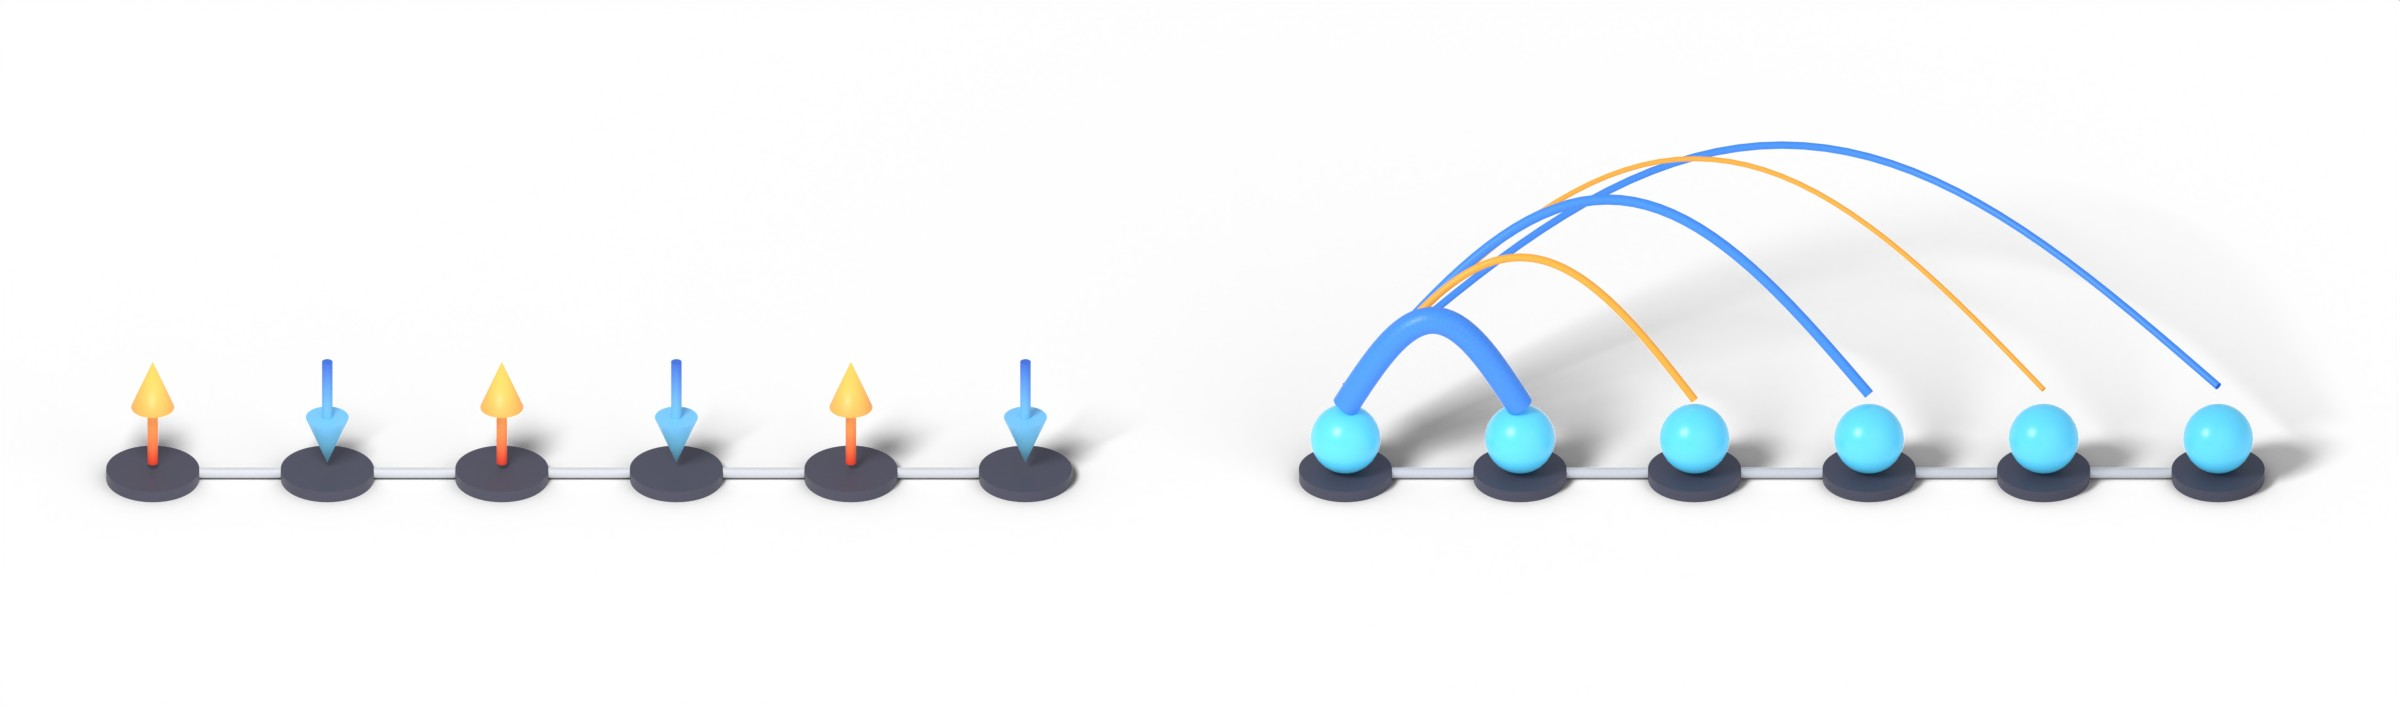
\includegraphics[width=\figw]{../blender/out/hubbard_moments.jpg}};
  %% written by figlib.py; x and y in units of the image width
\coordinate (a) at (0.0212\figw,0.2311\figw);
\coordinate (chainA) at (0.2455\figw,0.0704\figw);
\coordinate (b) at (0.5182\figw,0.2311\figw);
\coordinate (chainB) at (0.7424\figw,0.0704\figw);

  \node[lbl, font=\normalsize, anchor=west] at (a) {(a)\quad mean field};
  \node[lbl, font=\normalsize, anchor=west] at (b) {(b)\quad exact};
  \node[lbl, anchor=north] at (chainA) {$m_i=(-1)^i m$};
  \node[lbl, anchor=north] at (chainB) {$m_i=0$ on every site, arcs $\langle \mathbf S_0\cdot\mathbf S_j\rangle$};
\end{tikzpicture}
\end{document}
